  \documentclass[11pt, letterpaper]{report}
  \usepackage[utf8]{inputenc}
\usepackage{enumitem}
\usepackage{amsmath}
\usepackage{amssymb}
\usepackage{graphicx}
\usepackage{floatrow}
\usepackage{setspace}
\usepackage{etoolbox}
\usepackage{chngcntr}
\usepackage{titlesec}
\usepackage[margin=1in]{geometry}

\AtBeginEnvironment{quote}{\singlespacing\small}
\numberwithin{equation}{section}
\counterwithout{section}{chapter}
\newcommand{\norm}[1]{\left\lVert#1\right\rVert}

\titleformat{\chapter}{\normalfont\huge}{\thechapter}{20pt}{\huge\bfseries}

\title{TDT4171 - Artificial Intelligence Methods}
\author{Martin Bjerke}

\begin{document}

\maketitle

\tableofcontents

\vfill

In the following summary of the syllabus of TDT4171 in 2018, text that has an
additional margin is only mentioned in the syllabus, not in the lectures. The
sections and equations have the same numbering as in the book.

\chapter{Book}

\setcounter{section}{12}
\section{Quantifying Uncertainty}
Agent encounters uncertainty through partial obersvability, non-determinism or
both. To counter this problem-solving agents and logic agents tracks the world
sate and stores it as a \emph{belief state}. The \emph{qualification problem}
arises when an agent tries to store all possibilities(even implausible ones) in
its belief stat, making it impossible to infer its next action. Therefore
\emph{rational decision} takes into consideration both the relative importance
of an action and its likelihood.

Using inference to make an action fails on the following ground:
\begin{itemize}[label={}]
\item \emph{Laziness} failure to enumerate exceptions, qualifications etc
\item \emph{Theoretical ignorance} no theory for the domain
\item \emph{Practical ignorance} not possible to run all tests
\end{itemize}

Probabilistic assertions can summarise these effects, and an agent can store
its \emph{degrees of belief} that something will happen and use
\emph{probability theory} to chose the best
action. The combination of probability theory and \emph{utility
  theory}(inference) is called \emph{decision theory} and all of them can be
used to choose an action.

Probability gives an assertion about how the world looks(there is a 50\%
chance of rain today versus it is raining today), and the set of all possible
worlds(denoted $\Omega$) is called the sample space. A fully specified probability model gives a
probability, $P(\omega)$, of each possible world, and by the axioms of
probability each world has a probability between $0$ and $1$ and together the
probability must sum to 1:
\begin{equation}
  \label{eq:axioms}
  0 \leq P(\omega) \leq 1 \text{ for every } \omega \text{ and } \sum_{\omega \in
  \Omega} P(\omega) = 1
\end{equation}

The probability of \emph{propositions}(also called probabilistic assertions or queries,
or events) are the sum of the probability of the worlds where the proposition
holds:
\begin{equation}
  \label{eq:proposition}
  \text{For any proposition $\phi$, }P(\phi) = \sum_{\omega \in \phi} P(\omega)
\end{equation}


There are different ``types'' of probability:
\begin{itemize}[label={}]
\item \textbf{Prior/unconditional  probabilities: } Independent probabilities
\item \textbf{Posterior/conditional probabilities: } Dependent probabilities,
  the probability of rain, given that its already cloudy. Denoted $P(a \mid b)$.
\item \textbf{Probability distributions: } Outputs a probability given a value,
  most common in settings where the sample space is continuous, like temperature.
\item \textbf{Joint probability  distributions: } Normalised probability distributions
\end{itemize}
As more knowledge is gained, conditions arises, like you might not know you have
a cavity, but when you get toothache, you might consider it, $P(Cavity |
Toothache )$. Note, this means you ONLY know that you have a toothache, not
anything more relevant information. The conditional probability can be
calculated using unconditional probabilities:
\begin{equation}
  \label{eq:prodrule}
  P(a \mid b) = \frac{P(a \wedge b)}{P(b)} \text{ or usually presented as the \emph{product rule}}
  P(a \wedge b) = P(a \mid b)P(b)
\end{equation}

Some notation, \emph{random variables} are denoted with uppercase names and each
variable has a \emph{domain} of possible values, like $Die = \{1,2,3,4,5,6\}$,
boolean variables has two values $\{true, false\}$ and values with names are
denoted with lowercase names. When a bold $\boldsymbol{P}$ is used it the probability of all
the possible values of the variable, $\boldsymbol{P}(Weather) = \langle 0.6,0.1,
0.29, 0.01 \rangle$\footnote{Meaning here that $P(Weather = sunny) = 0.6$,
  $P(Weather = rain) = 0.1$, $P(Weather = cloudy) = 0.29$, and $P(Weather =
  snow) = 0.01$} and this is also called a \emph{probability distribution}. With
discrete variables the probability distribution can be represented as a
\emph{joint probability distribution} as shown below. Going back to the possible
worlds talk about above, if each random variable of a world is given a specific
value this represents one specific world. If the joint probability distribution
contains all possible random variables, then it is \emph{full joint probability distribution}(FJPD).

\begin{center}
  \begin{tabular}{|c|c|c|c|c|}
    \hline
    & \multicolumn{2}{|c|}{toothache} & \multicolumn{2}{|c|}{$\neg$ toothache} \\
    \hline
    & catch & $\neg$catch & catch & $\neg$catch \\
    \hline
    cavity       & .108 & .012 & .072 & .008 \\
    \hline
    $\neg$cavity & .016 & .064 & .144 & .576 \\
    \hline
  \end{tabular}
\end{center}
Using this table each possible value of each variable can be calculated using
probabilistic inference: ex.
$P(toothache) = .108 + .012 + .016 + 0.64 = .2$ and $P(cavity \vee
toothache) = .108 + .012 + .016 + .64 + .072 + .008 = .28$.

Together with the product rule (Eq. \ref{eq:unconditional}) and the
\emph{inclusion-exclusion principle} (Eq. \ref{eq:inc-exc}) we get the
\emph{Kolmogorov's axioms}. These build up the rest of probability theory.

\begin{equation}
  \label{eq:inc-exc}
  P(a \vee b) = P(a) + P(b) - P(a \wedge b)
\end{equation}

Summing up all the entries of a FJPD of a specific value, i.e $P(cavity) = .108
+ .012 + .072 + .008 = 0.2$, is called \emph{marginalisation} and can be
represented as the following general rule, with the variables $\boldsymbol{Y}$
and $\boldsymbol{Z}$:
\begin{equation}
  \label{eq:margin}
  \boldsymbol{P}(Y) = \sum_{z \in \boldsymbol{Z}} \boldsymbol{P}(Y,z)
\end{equation}

Above this is partially done with $Cavity$, $\boldsymbol{P}(Cavity) = \sum_{z
  \in \{Catch, Toothache\}}\boldsymbol{P}(Cavity, z)$. From Eq. \ref{margin} we
get the conditioning rule:

\setcounter{equation}{7}
\begin{equation}
  \label{eq:conditioning}
  \boldsymbol{P}(\boldsymbol{Y}) = \sum_{z}\boldsymbol{P}(\boldsymbol{Y} \mid z)P(z)
\end{equation}

Going back to Eq. \ref{eq:prodrule} and if you calculate both $P(cavity \mid
toothache) = 0.6$ and $P(\neg cavity \mid thoothache) = 0.4$ these add up to
1, as they should. Also notice that the $\frac{1}{P(toothache)}$ is constant,
and therefore we view it as a \emph{normalisation} constant of the distribution
of $\boldsymbol{P}(Cavity \mid toothache)$ and is therefore swapped with a
normalisation variable $\alpha$, which is set so that a distribution
$\boldsymbol{P}(A)$ has a total probability of 1. This is done since
$\frac{1}{P(toothache)}$ is just a normalisation, so we don't actually need to
know it. From this we extract a general inference procedure:

Let $X$ be all the query variables, $E$ be the evidence variables and $e$ be the
specific values and let $Y$ be the remaining hidden variables. This gives the
following formula for summing the joint entries:
\begin{equation}
  \label{eq:inference}
  \boldsymbol{P}(X \mid e) = \alpha \boldsymbol{P}(X,e) = \alpha \sum_y \boldsymbol{P}(X,e, y)
\end{equation}

In mote cases, the use of conditional independence reduces the size of the
representation of the joint distribution from exponential in n to linear. For
example n coin flips, if they where dependent there would be $2^n$
representations in the joint distribution, but since they are independent, only
$n$ is needed.

Identifying independence, two variables are independent iff: \\
$P(X \mid Y) = P(X)$ equivalently $P(Y \mid X) = P(Y)$

Bayes rule:
\setcounter{equation}{12}
\begin{equation}
\begin{split}
  \label{eq:bayesrule}
  \boldsymbol{P}(Y \mid X) &= \frac{\boldsymbol{P}(X \mid
   Y)\boldsymbol{P}(Y)}{\boldsymbol{P}(X)} \\
  & \text{or with some background evidence $e$} \\
  \boldsymbol{P}(Y \mid X,e) &= \frac{\boldsymbol{P}(X \mid Y,e)\boldsymbol{P}(Y,e)}{\boldsymbol{P}(X,e)} \\
  & \text{or by using the normalisation trick from before} \\
  \boldsymbol{P}(X \mid e) &= \alpha \langle P(e \mid x)P(x), P(e \mid \neg x)P(\neg x) \rangle \\
  &= \boldsymbol{P}(X \mid Y) = \alpha \boldsymbol{P}(Y \mid X)\boldsymbol{P}(X)
\end{split}
\end{equation}

Variables are said to be conditionally independent if they have the same \emph{cause},
but different \emph{effects}, where the effects are independent, but they are both
dependent on the cause. I.e. Toothache and catch are both an effect of having a
cavity, but having a toothache is independent of the toothpick to catch and vise versa;
$\boldsymbol{P}(toothache \wedge catch \mid Cavity) =
\boldsymbol{P}(toothache \mid Cavity) \boldsymbol{P}(catch \mid Cavity) $.
Conditional independence is represented in the following equation:
\setcounter{equation}{18}
\begin{equation}
  \begin{split}
    \label{eq:contional}
    \boldsymbol{P}(X, Y \mid Z) &= \boldsymbol{P}(X \mid Z)\boldsymbol{P}(Y \mid Z) \\
    &\text{since Y and X are independent, the following is also true} \\
    \boldsymbol{P}(X \mid Y, Z) &= \boldsymbol{P}(X \mid Z) \\
    \boldsymbol{P}(Y \mid X, Z) &= \boldsymbol{P}(Y \mid Z) \\
  \end{split}
\end{equation}

Using conditional independence to ``shorten'' a probability distribution is
called a \emph{naive Bayes model}, this is because it used in cases where the
effect variables are not actually conditionally independent given the cause
variable.

\section{Bayesian networks}

% Motivation: \\
% Hard to find independence and conditional independence by only looking at the
% raw data, however, using background knowledge of the data, one can construct
% hypotheses about independence and conditional independence, which are easy to
% check.

Bayesian networks are graphical notations for conditional independence
assertions, giving a compact specification of full joint distributions.
The syntax is a set of nodes(one per variable) that makes out a DAG and a conditional
distribution for each node given its parents, $\boldsymbol{P}(X_i \mid Parents(X_i))$

All conditional distribution represented as a conditional probability
table(CPT) gives the distribution over $X_i$ for each combination of parent
values.

Example: A CPT for boolean $X_i$ with k boolean parents has $2^k$ rows for the
combinations of parent values. Since $X_i$ is boolean, $P(X_i = true) = 1 - P(X_i
= false)$, so each row requires only one representative, so if each variable has
maximum k parents, the complete network requires $O(n \cdot 2^k)$ numbers.

\subsection*{Representing a full joint distribution and constructing a Bayesian network}

A generic entry in a joint distribution is just a conjunction of assignment of
values to all variables, $P(X_1 = x_1 \wedge X_2 = x_2 \wedge ... \wedge X_n =
x_n)$ which is written in shorthand as $P(x_1, x_2,...,x_n)$. Since $x_i$ is
just dependent of its parents this value is given by:
\begin{equation}
  \label{eq:parents}
  P(x_1, x_2,..., x_n) = \prod_{i=0}^n P(x_i \mid parents(X_i))
\end{equation}

Example: Let B and E be parents of A, and J and M be children of A,
\begin{equation}
    P(j \wedge m \wedge a \wedge \neg b \wedge \neg e) =
    P(j \mid a)P(m \mid a)P(a \mid \neg b, \neg e)P(\neg b)P(\neg e)
\end{equation}

The chain rule can be extracted from this using the product rule:
\begin{equation}
  \begin{split}
    \label{eq:chainrule}
    P(x_1,...,x_n) &= P(x_n \mid x_{n-1},...,x_1)P(x_{n-1},...,x_1) \\
      &= P(x_n \mid x_{n-1},...,x_1)P(x_{n-1} \mid x_{n-2},...,x_1)P(x_{n-2},...,x_1) \\
      &= ... = \prod_{i=1}^n P(x_i \mid x_{i-1},...,x_1) \\
  \end{split}
\end{equation}

Using the chain rule in Eq. \ref{eq:parents} and generalising:
\begin{equation}
  \label{eq:parentsgen}
  \boldsymbol{P}(X_i \mid X_i,...,X_1) = \boldsymbol{P}(x_i \mid Parents(X_i))
\end{equation}

Local semantics: each node is conditionally independent of its non descendants
given its parents.
Markov blanket: Each node is conditionally independent of all other nodes then its
parents, children and children's parents.

Construction of a Bayesian network:
\begin{enumerate}
  \item Choose an ordering of variables $X_1,...,X_n$
  \item for $i = 1$ to $n$
    \begin{enumerate}
      \item add $X_i$ to the network
      \item select parents from $X_1,...,X_{i-1}$ such that $P(X_i \mid
        Parents(X_i)) = P(X_i \mid X_1,...,X_{i-1})$
    \end{enumerate}
\end{enumerate}

\begin{enumerate}[label=Step \arabic* - ]
  \item Decide what to model
  \item Define variables
  \item Define the graphical structure that connects the variables(The
    qualitative part)
  \item Fix parameters to specify each $P(x_i \mid pa(x_i))$(The quantitative
    part)
  \item Verification
\end{enumerate}

There are other approaches, other then probability, to handle uncertainty:
\begin{itemize}
\item Qualitative reasoning: I.e. default reasoning: A conclusion is sound as
  long as there are no better conclusions to draw.
\item Rule-based: Add a ``fudge factor'' to each rule to accommodate
  uncertainty. There are 3 desirable properties from rule-based:
  \begin{itemize}
  \item \emph{Locality}; Given the rule $A \implies B$, B can be concluded by
    only looking at A, not the other evidence.
  \item \emph{Detachment}; Once a proof for a proposition is found it can be
    detached from its justification.
  \item \emph{Truth-functionality}; Truth of sentences can be computed by the
    truth of the components. This can't be done in probability without independence.
  \end{itemize}
  There have been attempts to add uncertainty to RB by assigning a belief to the rules.
\item Dempster-Shafer theory: Compute the probability that the evidence supports
  the proposition(use a \emph{belief function}).
\item Fuzzy logic: is fuzzy
\end{itemize}

\section{Probabilistic reasoning over time}
To handle the coming dynamic models they are viewed discretely using \emph{time
  slices}, containing sets of observable and unobservable random variables. For
notation $\boldsymbol{X}_t$ denotes the set of state variables at time $t$ which
are unobservable and $\boldsymbol{E}_t$ denotes the set of observable evidence
variables, so the observations at time $t$ are $\boldsymbol{E}_t = e_t$. The
notation a:b denotes (inclusive) the interval from a to b, so
$\boldsymbol{X}_{a:b}$ are the set of variables
$\boldsymbol{X}_a,...,\boldsymbol{X}_b$. The examples used are based on the
umbrella world of Chapter 15. The notations of \emph{transition model} is how
the world evolves and \emph{sensor model} is how the evidence variables get
their values.

The \emph{transition model} specifies the probability distribution over the
latest state variables, given the previous states,
$\boldsymbol{P}(\boldsymbol{X}_t \mid \boldsymbol{X}_{0:t-1})$. Using this
increases the number of previous states need over time. This is solved by making
a \emph{Markov assumption}, the next states only depend on a finite set of
previous states. This is called a \emph{Markov process} or \emph{Markov chain},
the simplest form being the \emph{first-order Markov process} where the current
state only depends on the previous one. In other words, a future state is
only dependent on the previous state and conditionally independent of the rest:
\begin{equation}
  \label{eq:first-order markov}
  \boldsymbol{P}(\boldsymbol{X}_t \mid \boldsymbol{X}_{0:t-1}) = \boldsymbol{P}(\boldsymbol{X}_t \mid \boldsymbol{X}_{t-1})
\end{equation}

Having bounded the number of transition models using a Markov assumption, we
want to bound the possible number of different transition models that arises. We
want a \emph{stationary process}, where the rules of changes to the world states
does not change. I.e in the umbrella world $\boldsymbol{P}(R_t \mid R_{t-1})$ is
the same for all $t$.

Next is bounding the sensor model. This is done by making a \emph{sensor Markov
  assumption} that works the same way as a Markov assumption, limiting the
number of past evidence values needed and giving us the following sensor
model(sometimes called the \emph{observation model}):
\begin{equation}
  \label{eq:sensor markov}
  \boldsymbol{P}(\boldsymbol{E}_t \mid \boldsymbol{X}_{0:t}, \boldsymbol{E}_{0:t-1})
  = \boldsymbol{P}(\boldsymbol{E}_t \mid \boldsymbol{X}_{t})
\end{equation}

Lastly we need a prior probability distribution at time $t = 0,
\boldsymbol{P}(\boldsymbol{X}_0)$. Given these assumptions and equations we have
the complete joint distribution for any t:
\begin{equation}
  \label{eq:complete joint dist}
  \boldsymbol{P}(\boldsymbol{X}_{0:t}, \boldsymbol{E}_{1:t}) =
  \boldsymbol{P}(\boldsymbol{X}_0) \prod_{i=1}^t\boldsymbol{P}(\boldsymbol{X}_i \mid \boldsymbol{X}_{i-1})\boldsymbol{P}(\boldsymbol{E}_i \mid \boldsymbol{X}_{i})
\end{equation}

To use these models, the following interference tasks can be used:
\begin{itemize}
\item \emph{Filtering}: Calculate the posterior distribution, aka the belief
  state, given the evidence observed so up until a time slice $t$;
  $\boldsymbol{P}(\boldsymbol{X}_t \mid \boldsymbol{e}_{1:t})$. A close related
  calculation can be done to get $P(\boldsymbol{e}_{1:t})$
\item \emph{Prediction}: Calculate the probability of a future belief state at
  time slice $k$, where $k > 0$, given the present evidence values;
  $\boldsymbol{P}(\boldsymbol{X}_{t+k} \mid \boldsymbol{e}_{1:t})$.
\item \emph{Smoothing}: Calculate the belief state of a previous time slice $k$,
  given the observed evidence up until $t$, where $0 < k < t$;
  $\boldsymbol{P}(\boldsymbol{X}_{k} \mid \boldsymbol{e}_{1:t})$.
\item \emph{Most likely explanation}: Calculate the most likely belief states
  that would give the observed evidence;
  $argmax_{x_{1:t}}P(x_{1:t} \mid e_{1:t})$
\end{itemize}
Together with these tasks learning is also possible. Both the transition model
and the sensor model can be learned through observation.

\subsection*{Filtering/forward message}
To calculate the belief state at time slice $t+1$, we can use the following
equation;
\begin{equation}
  \begin{split}
    \label{eq:filtering}
    \boldsymbol{P}(\boldsymbol{X}_{t+1} \mid \boldsymbol{e}_{1:t+1}) &=
      \boldsymbol{P}(\boldsymbol{X}_{t+1} \mid \boldsymbol{e}_{1:t}, \boldsymbol{e}_{t+1}) \\
    &= \alpha \boldsymbol{P}(\boldsymbol{e}_{t+1} \mid \boldsymbol{X}_{t+1}, \boldsymbol{e}_{1:t})
      \boldsymbol{P}(\boldsymbol{X}_{t+1} \mid \boldsymbol{e}_{1:t}) \\
    &= \alpha \boldsymbol{P}(\boldsymbol{e}_{t+1} \mid \boldsymbol{X}_{t+1})
     \boldsymbol{P}(\boldsymbol{X}_{t+1} \mid \boldsymbol{e}_{1:t})
  \end{split}
  \begin{split}
    &\text{(dividing up the evidence)}\\
    &\text{(using Bayes rule)} \\
    &\text{(using sensor Markov assumption)}
  \end{split}
\end{equation}
The terms are as follows; $\alpha$, the normalisation constant;
$\boldsymbol{P}(\boldsymbol{e}_{t+1} \mid \boldsymbol{X}_{t+1})$, the sensor
model is used to update the belief state;
$\boldsymbol{P}(\boldsymbol{X}_{t+1} \mid \boldsymbol{e}_{1:t})$, a prediction
of the next belief state. This last prediction is based on the current belief
state $\boldsymbol{X}_t$ and this is used integrated in the following way:
\begin{equation}
  \label{eq:filtering2}
  \begin{split}
    \boldsymbol{P}(\boldsymbol{X}_{t+1} \mid \boldsymbol{e}_{1:t+1}) &=
    \alpha \boldsymbol{P}(\boldsymbol{e}_{t+1} \mid \boldsymbol{X}_{t+1})
    \sum_{\boldsymbol{x}_t} \boldsymbol{P}(\boldsymbol{X}_{t+1} \mid \boldsymbol{x}_t,
    \boldsymbol{e}_{1:t}) P(\boldsymbol{x}_t \mid \boldsymbol{e}_{1:t}) \\
    &= \alpha \boldsymbol{P}(\boldsymbol{e}_{t+1} \mid \boldsymbol{X}_{t+1})
    \sum_{\boldsymbol{x}_t} \boldsymbol{P}(\boldsymbol{X}_{t+1} \mid \boldsymbol{x}_t)
    P(\boldsymbol{x}_t \mid \boldsymbol{e}_{1:t})
  \end{split}
  \begin{split}
    &\text{(predicting $\boldsymbol{X}_{t+1}$ using $\boldsymbol{X}_t$)} \\
    &\text{(using Markov assumption)}
  \end{split}
\end{equation}
Notice that $\boldsymbol{P}(\boldsymbol{X}_{t+1} \mid \boldsymbol{x}_t)$ comes
from the transition model. Further $\boldsymbol{P}(\boldsymbol{x}_t \mid
\boldsymbol{e}_{1:t})$ can be viewed as a \emph{forward message}(as this is calculated at each
time step using the previous state) and Eq. \ref{eq:filtering2} can be in
shorthand as:
\[\boldsymbol{f}_{1:t+1} = \alpha FORWARD(\boldsymbol{f}_{1:t},\boldsymbol{e}_{1:t+1})\]
where $\boldsymbol{f}_{1:0} = \boldsymbol{P}(\boldsymbol{X}_0)$

\subsection*{Prediction}
This is done by using Eq. \ref{eq:filtering2} using just the evidence observed
so far, $\boldsymbol{e}_{1:t}$ and the previous predicted state, $\boldsymbol{X}_{t+k}$:
\begin{equation}
  \label{eq:prediction}
  \boldsymbol{P}(\boldsymbol{X}_{t+k+1} \mid \boldsymbol{e}_{1:t}) =
  \sum_{\boldsymbol{x}_{t+k}} \boldsymbol{P}(\boldsymbol{X}_{t+k+1} \mid \boldsymbol{x}_{t+k})
  P(\boldsymbol{x}_{t+k} \mid \boldsymbol{e}_{1:t})
\end{equation}
These predictions will converge to a fixed sate called the \emph{stationary
  distribution} after a number of time steps called the \emph{mixing time},
dooming any attempt to predicting to far into the future.

\subsection*{Likelihood}
This is useful when reviewing the assumed belief states calculated given the
evidence and is done using the \emph{likelihood message},
$\boldsymbol{l}_{1:t}(\boldsymbol{X}_t) = \boldsymbol{P}(\boldsymbol{X}_t,
\boldsymbol{e}_{1:t})$, this in turn can be inferred into the following:
  \begin{gather}
  \label{eq:likelihood}
  \boldsymbol{l}_{1:t+1} = FORWARD(\boldsymbol{l}_{1:t}, \boldsymbol{e}_{1:t+1})
  \nonumber\\
  \text{and from $\boldsymbol{l}_{1:t}$ the actual likelihood can be calculated} \\
  L_{1:t} = P(\boldsymbol{e}_{1:t}) = \sum_{\boldsymbol{x}_t}
  \boldsymbol{l}_{1:t}(\boldsymbol{x}_t) \nonumber
  \end{gather}

\subsection*{Smoothing}
Computing the belief state of a previous state, $\boldsymbol{P}(\boldsymbol{X}_k
\mid \boldsymbol{e}_{1:t})$ at time $0 \leq k \leq t$, using evidence up to the
present, $t$, can be done by splitting the computation into two:
\begin{equation}
  \label{eq:smoothing}
  \begin{split}
    \boldsymbol{P}(\boldsymbol{X}_k \mid \boldsymbol{e}_{1:t}) &=
    \boldsymbol{P}(\boldsymbol{X}_k \mid \boldsymbol{e}_{1:k}, \boldsymbol{e}_{k+1:t}) \\
    &= \alpha \boldsymbol{P}(\boldsymbol{X}_k \mid \boldsymbol{e}_{1:k})
    \boldsymbol{P}(\boldsymbol{e}_{k+1:t} \mid \boldsymbol{X}_k, \boldsymbol{e}_{1:k}) \\
    &= \alpha \boldsymbol{P}(\boldsymbol{X}_k \mid \boldsymbol{e}_{1:k})
    \boldsymbol{P}(\boldsymbol{e}_{k+1:t} \mid \boldsymbol{X}_k) \\
    &= \alpha \boldsymbol{f}_{1:k} \times \boldsymbol{b}_{k+1:t}
  \end{split}
  \begin{split}
    &\text{split the evidence} \\
    &\text{using Baye's rule} \\
    &\text{using Eq. \ref{eq:sensor markov}} \\
    &\text{element wise multiplication} \\
  \end{split}
\end{equation}
Where $\boldsymbol{b}_{k+1:t} = \boldsymbol{P}(\boldsymbol{e}_{k+1:t} \mid
\boldsymbol{X}_k)$ is the backward message that is the recursive analogy to the
forward message that is calculated backwards from $t$:
\begin{equation}
  \label{eq:backward}
  \begin{split}
    \boldsymbol{P}(\boldsymbol{e}_{k+1:t} \mid \boldsymbol{X}_k) &=
    \sum_{\boldsymbol{x}_k+1} \boldsymbol{P}(\boldsymbol{e}_{k+1:t} \mid \boldsymbol{x}_{k+1},\boldsymbol{X}_{k})
    \boldsymbol{P}(\boldsymbol{x}_{k+1} \mid \boldsymbol{X}_{k}) \\
    &= \sum_{\boldsymbol{x}_k+1} \boldsymbol{P}(\boldsymbol{e}_{k+1:t} \mid \boldsymbol{x}_{k+1})
    \boldsymbol{P}(\boldsymbol{x}_{k+1} \mid \boldsymbol{X}_{k}) \\
    &= \sum_{\boldsymbol{x}_k+1} \boldsymbol{P}(\boldsymbol{e}_{k+1},\boldsymbol{e}_{k+2:t} \mid
    \boldsymbol{x}_{k+1}) \boldsymbol{P}(\boldsymbol{x}_{k+1} \mid \boldsymbol{X}_{k}) \\
    &= \sum_{\boldsymbol{x}_k+1} \boldsymbol{P}(\boldsymbol{e}_{k+1} \mid
    \boldsymbol{x}_{k+1}) \boldsymbol{P}(\boldsymbol{e}_{k+2:t} \mid
    \boldsymbol{x}_{k+1}) \boldsymbol{P}(\boldsymbol{x}_{k+1} \mid \boldsymbol{X}_{k}) \\
  \end{split}
  \begin{split}
    &\text{conditioning on $\boldsymbol{X}_{k+1}$}\\
    &\text{conditional independence} \\
  \end{split}
\end{equation}
Notice that the first and third products are from the models, and the second is
the recursive call.

\subsection*{Most likely sequence}
Because of the \emph{Markov assumptions} the transition between states are
dependent on the previous state, therefore, if you change the question from
which sequence is most likely to what path through the states that takes(see Fig
15.5 in book), the most likely state at time $t+1$ is dependent on the most
likely state at $t$. This relationship can be expressed as:
\begin{equation}
  \label{eq:mostlikely}
  \begin{split}
  &\max_{\boldsymbol{x}_1...\boldsymbol{x}_t} \boldsymbol{P}(\boldsymbol{x}_1,...,\boldsymbol{x}_t,\boldsymbol{X}_{t+1}
  \mid \boldsymbol{e}_{1:t+1}) = \\
  &\alpha \boldsymbol{P}(\boldsymbol{e}_{1:t+1} \mid \boldsymbol{X}_{t+1}) \max_{\boldsymbol{x}_t}
  (\boldsymbol{P}(\boldsymbol{X}_{t+1} \mid \boldsymbol{x}_t)
  \max_{\boldsymbol{x}_1...\boldsymbol{x}_{t-1}} P(\boldsymbol{x}_1,...,\boldsymbol{x}_{t} \mid \boldsymbol{e}_{1:t}) ) \\
  \end{split}
\end{equation}

The \emph{Hidden Markov Model}(HMM) is a way to represent the world state as a
single discrete random variable, where the values are the possibles states of
the world. This will be the state variable $X_t$, which is a vector of the size
$S$, where $S$ is the number of possible states of the world. The
\emph{transition model} $\boldsymbol{P}(X_t \mid X_{t-1})$ is written as a
$S \times S$ matrix $\boldsymbol{T}$, where $\boldsymbol{T}_{ij} = P(X_t = j \mid
X_{t-1} = i)$, the transition from state $i$ to state $j$. Next the sensor model
is written as a diagonal matrix $\boldsymbol{O}$, where the diagonal $\boldsymbol{O}_{i} =
P(e_t\mid X_t = i)$ and the rest are 0. The forward and backward messages then
becomes:
\begin{gather}
  \label{eq:hmm}
  \boldsymbol{f}_{1:t+1} = \alpha \boldsymbol{O}_{t+1}\boldsymbol{T}^T\boldsymbol{f}_{1:t} \\
  \boldsymbol{b}_{k+1:t} = \boldsymbol{T}\boldsymbol{O}_{k+1}\boldsymbol{b}_{k+2:t}
\end{gather}

In the real world there are often failures in the observable variables, like a
sensor failing, both temporally and permanently. These event can be handled
using \emph{Dynamic Bayesian Networks}(DBN) which incorporates several different models:
\begin{itemize}
\item \emph{Transient failure model}: This model handles the event of a
  temporary error in the observable variable by adding a small probability that
  the wrong value might be observed.
\item \emph{Persistent failure model}: This model handles the event when the
  the observable variable permanently return the wrong value. This is done by
  adding a new variable to the DBN that represents the state of the sensor of
  that observable variable.
\end{itemize}

\section{Making simple decisions}
When dealing with decisions we define $RESULT(a)$ as a random variable whose
values are possible outcome states. The probability of outcome $s'$ of an action
$a$ given evidence $\boldsymbol{e}$ is written as: $P(RESULT(a)=s' \mid
a,\boldsymbol{e})$. An agents preference is captured by the \emph{utility
  function}, $U(s)$, and the \emph{expected utility} of an action given
evidence, $EU(a \mid \boldsymbol{e})$, is just the average utility value of the
possible outcomes:
\begin{equation}
  \label{eq:expectedutil}
  EU(a \mid \boldsymbol{e}) = \sum_{s'} P(RESULT(a)=s' \mid a,\boldsymbol{e})U(s')
\end{equation}

The principle of \emph{maximum expected utility}(MEU) says that a rational agent
should choose the action that maximises the agent's expected utility; $action =
\text{argmax}_a EU(a \mid \boldsymbol{e})$
Note that the utility score is not the same as the performance score, as the
utility score is the expected value of an action, the performance score is the
actual value of the action. For an agent to be \emph{unbiased} the difference of
expected value and predicted value must be 0.

Some notation on preference:
\begin{itemize}
\item[A $\prec$ B] A is preferred over B
\item[A $\sim$ B] A and B are equally preferred
\item[A $\precsim$ B] A is preferred over B or they are equal
\end{itemize}
The probability of the outcomes of an action is represented as a lottery $L$
with each outcome state, $S_1,...,S_n$, and their probabilities, $p_1,...,p_n$;
$L = [p_1,S_1;p_2,S_2;...;p_n,S_n]$.

For a preference relation to be reasonable it must fulfil the following
restraints:
\begin{itemize}
\item \emph{Orderability:} Exactly one of the following must hold;
  $(A \prec B), (B \prec A), (A \sim B)$ \\
  The sates must either be equal or one can order them.
\item \emph{Transitivity:} $(A \prec B) \wedge (B \prec C) \implies (A \prec
  C)$
\item \emph{Continuity:} $A \prec B \prec C \implies \exists p [p,A; 1-p,C] \sim
  B$ \\
  There must be a way to ``represent'' the outcome of B, by using A and B.
\item \emph{Substitutability:} $A \sim B \implies [p,A; 1-p,C] \sim [p,B;
  1-p,C]$ \\
  Here $\sim$ can be swapped with $\prec$.
\item \emph{Monotonicity:} $ A \prec B \implies (p > q \iff [p,A; 1-p,B] \prec
  [q,A;1-q,B]) $ \\ If A is preferred over B, then the lottery with the highest
  probability of getting A is preferred.
\item \emph{Decomposability:} $[p,A;1-p,[q,B;1-q,C]] \sim
  [p,A;(1-p)q,B;(1-p)(1-q),C]$ \\ Two consecutive lotteries can be turned into one.
\end{itemize}

Some utility function properties:
\begin{itemize}
\item $U(A) < U(B) \iff A \prec B$
\item $U(A) = U(B) \iff A \sim B$
\item The utility of a lottery is defined as: \\
  $ U(L) = U([p_1,S_1;p_2,S_2;...;p_n,S_n]) = \sum_i p_iU(S_i)$
\end{itemize}
As an agent might only be interested in ordering states, the actual utility
value isn't necessary, these functions are called \emph{value functions} or
\emph{ordinal utility functions}. \emph{Preference elicitation} is used to
discover a utility function and is done by presenting choices to an agent the
using its observed preferences.

When an agent prefers to take risks for higher reward they are
\emph{risk-seeking}, the reverse is \emph{risk-averse}, preferring safer bets.
The value an agent accepts as guaranteed after a bet is the \emph{certainty
  equivalent}, the difference between this end the \emph{ expected monetary value }(EMV)
is the \emph{insurance premium}.

\emph{Normative theory} is the theory of how an agent should act, and
\emph{descriptive theory} is the theory of how the agent actually acts. Not all
actions are completely rational as covered by the \emph{certainty effect}, that
a person usually chooses the guaranteed win. Something similar is covered by the
\emph{ambiguity aversion}, that people go for the known probabilities, instead
of the unknown probabilities.

Problems where the utility is based on several variables are called
\emph{multiattribute utility theory}. Here the terms \emph{strict dominance}
means that a solution $S_1$ is better in every utility aspect than an solution
$S_2$, and \emph{stochastic dominance}, if two actions, $A_1, A_2$ leads to probability
distributions $p_1(x),p_2(x)$ the $A_1$ stochastic dominates $A_2$ if:
$\forall x \int_{-\infty}^x p_1(x')dx' \leq \int_{-\infty}^x p_2(x')dx'$.

\emph{Preference independence} is when two variables are not dependent on the
value of a third variable. \emph{Mutual preferential independence} (MPI) says
that each variable is equally important, so they don't affect the other
variables during a trade off. For attributes that are MPI the preferred
behaviour can be described by maximising the function \emph{additive value function},
$V(x_1,...,x_n) = \sum_i V_i(x_i)$. The preference independence can be extended
with \emph{utility independence}(UI) to cover lotteries. A set of attributes is
\emph{mutually utility independent} (MUI) if each of its subsets is UI of the
remaining attributes. MUI can be expressed using a \emph{multiplicative utility function}.

Rational decisions can be done using decision networks, an extension of Bayesian
networks. The network is constructed by the following node types:
\begin{itemize}
\item \emph{Chance nodes:} same as for Bayesian networks, circles with variables
\item \emph{Decision nodes:} rectangles representing where the decision maker
  can take actions
\item \emph{Utility nodes:} diamonds representing the utility function.
\end{itemize}
These networks can be evaluated in the following way:

\begin{enumerate}
\item Set the evidence variables for the current state.
\item For each possible value of the decision node:
  \begin{enumerate}
  \item Set the decision node to that value.
  \item Calculate the posterior probabilities for the parent nodes of the
    utility node, using a standard probabilistic inference algorithm
  \item Calculate the resulting utility for the action.
  \end{enumerate}
\item Return the action with the highest utility.
\end{enumerate}

In information value theory the \emph{value of perfect information}(VPI) is
expressed as the following:
\[VPI_{ \boldsymbol{e} } (E_j) = (\sum_k P(E_j=e_{jk} \mid \boldsymbol{e})
  EU(\alpha_{e_{jk}} \mid \boldsymbol{e}, E_j = e_{jk}) ) - EU(\alpha \mid \boldsymbol{e}) \]
Where $Ej$ is the variable we don't know but want to find out, $\boldsymbol{e}$
is the observations so far, $e_{jk}$ is the new evidence and $\alpha$ is the value of the current best action.

Lastly in decision-theoretic expert systems \emph{decision analysis} studies the
application of decision theory on actual decision problems. There are usually
talk about two roles, the \emph{decision maker} that states preferences about
outcomes, and the \emph{decision analyst} that enumerates the possible actions
and outcomes and elicits preferences from the decision maker to determine the
best action. A decision-theoretic expert system is created in the following way:
\begin{enumerate}
\item \emph{Create a causal model:} determine all possible variables, utility
  functions and actions.
\item \emph{Simplify to a qualitative decision model:} Remove variables that
  does not affect the choice of action.
\item \emph{Assign probabilities}
\item \emph{Assign utilities:} These can be enumerated from the probabilities
\item \emph{Verify and refine the model:} Using a \emph{gold
    standard}(validation set)
\item \emph{Perform sensitivity analysis:} If small changes results in big
  changes in the chosen action, the system might not be ready.
\end{enumerate}

\section{Making complex decisions}
Focuses on \emph{sequential decision problems} where the utility function
depends on a sequence of decisions. First we look at the environment as \emph{fully
  observable}, that is has a \emph{transition model}, $P(s' \mid a,s)$ and that
the transitions are \emph{Markovian}. For each state an agent receives a reward
$R(s)$ depending on that state and the utility function is just the sum of these
rewards for the \emph{environment history}. This is called a \emph{Markov
  decision problem}(MDP).

When adding uncertainty to actions, i.e. there is a probability to take a right
instead of a left, a sequence of actions does not guarantee success, therefore
only the optimal action at each state is stored, $\pi(s)$, called a
\emph{policy}. The \emph{optimal policy} for a state is the policy that gives
the highest expected utility. As the performance of an agent is based on the
states it visited this becomes a story in \emph{ multiattribute utility theory}.
There is also the properties of \emph{finite} or \emph{infinite horizon}, where
the agent either must reach a terminate state after $N$ states, or has no such
constriction, on wards the an infinite horizon is assumed. If the optimal policy in a
state, $\pi^\ast(s)$, changes over time it is \emph{nonstationary}, and if it
does not it is \emph{stationary}. If an agent is stationary for preference it
has the same preference-order for $[s_0,s_1,s_2,...]$ and
$[s'_0,s'_1,s'_2,...]$, as for $[s_1,s_2,...]$ and $[s'_1,s'_2,...]$ iff $s_0=s'_0$.

If a system is stationary the following utility function can be assigned:
\begin{enumerate}
\item \emph{Additive rewards:} $U_h([s_0,s_1,s_2,...]) = \sum_{i=0} R(s_i)$
\item \emph{Discounted rewards:} $U_h([s_0,s_1,s_2,...]) = \sum_{i=0}
  \gamma^i R(s_i)$ \\ Here $0 < \gamma \leq 1$ is the \emph{discount factor},
  this also gives an interest rate of $(1/\gamma)-1$.
\end{enumerate}
When assuming the infinite horizon these functions become tricky as they both go
on to plus/minus infinity and we then have to order infinities. There are three
solutions to this:
\begin{enumerate}
\item \emph{Discounted rewards:} If $\gamma < 1$ this is infinite geometric
  series, which is finite: \\
  $U_h([s_0,s_1,s_2,...]) = \sum_{i=0}^\infty \gamma^i R(s_i) \leq
  \sum_{i=0}^\infty \gamma^i R_{\max} = R_{ \max } /(1-\gamma)$
\item \emph{Proper policy:} This requires there to be a terminate state, so
  infinite series are never encountered.
\item \emph{Average reward:} Averaging the rewards gives a way to handles the
  infinities.
\end{enumerate}
Note, discounted rewards are the best.

Let the random variable $S_t$ denote the state the agent reaches at time step
$t$ when using policy $\pi$. the expected utility then becomes:
\setcounter{equation}{1}
\begin{equation}
  \label{eq:expectedpolicyutil}
  U^\pi(s) = E[\sum_{t=0}^\infty \gamma^tR(S_t)]
\end{equation}
Next let $\pi^\ast_s$ denote the optimal policy of state $s$, and it is chosen
by:
\begin{equation}
  \label{eq:optimalpolicy}
  \pi^\ast_s = \text{argmax}_\pi U^\pi(s)
\end{equation}
And the best action can be calculated by:
\begin{equation}
  \label{eq:bestaction}
  \pi^\ast(s) = \text{argmax}_{a \in A(s)} \sum_{ s' } P(s' \mid s,a)U(s')
\end{equation}

To calculate the optimal utility one of two algorithms can be used; \emph{value
  iteration} or \emph{policy iteration}. The value iteration algorithm is based
on the \emph{Bellman equation}, these also give unique solutions:
\begin{equation}
  \label{eq:bellmaneq}
  U(s) = R(s) + \gamma \max_{a \in A(s)} \sum_{s' \in NEIGH(s)} P(s' \mid s,a)U(s')
\end{equation}
These equations are non linear and must therefore be solved using non-regular
methods, one is iterative where each state value is updated for each iteration
by the \emph{Bellman update}:
\begin{equation}
  \label{eq:bellmanupdate}
  U_{i+1} \leftarrow R(s) + \gamma \max_{a \in A(s)} \sum_{s' \in NEIGH(s)} P(s' \mid s,a)U_i(s')
\end{equation}
By showing that the Bellman update is a \emph{contraction} we guarantee that the
value iteration converges. There are two properties of a contraction function;
it has only one fixed point and for all inputs to the function, the output is
closer to the fixed point. By viewing the Bellman update as a operator $B$ and
$U_i, U_i'$ as vectors of utilities at iteration $i$, $U$ as the true utilities and the max norm of a vector
$\norm{U} = \max_s \mid U(s) \mid$ it can be shown that value
iteration converges:
\begin{equation}
  \label{eq:contration}
  \begin{split}
    \norm{BU_i - BU_i'} \leq \gamma \norm{U_i - U_I'} \\
    \norm{BU_i - U} \leq \gamma \norm{U_i - U} \\
  \end{split}
  \quad
  \begin{split}
    &\text{$B$ is an contraction of factor $\gamma$} \\
    &\text{using that $BU = U$ it shows that for each iteration} \\
    &\text{the error is reduced by at least $\gamma$} \\
  \end{split}
\end{equation}
From this it is also possible to calculate number of iterations needed to reach
an error of size $\epsilon$; $N = \lceil {\log (2R_{\max}/\epsilon
  (1-\gamma))/log(1/\gamma)} \rceil $ \\
Through contraction it is also shown that if the update is small then the
error is also small; $\norm{U_{i+1}-U_i} < \epsilon(1-\gamma)/\gamma \implies
  \norm{U_{i+1} - U} < \epsilon $ \\
Further the \emph{policy loss} is connected to error by the following, where
$U^{\pi_i}$ is the policy if $\pi_i$ was executed:
$\norm{U_i-U} < \epsilon \implies \norm{U^{\pi_i}-U} < 2\epsilon\gamma/(1-\gamma)$

Next we look at the \emph{policy iteration} that contains two steps:
\begin{enumerate}
\item \emph{Policy evaluation:} given a policy $\pi_i$, calculate the utility of
  each state if $\pi_i$ was executed,$U_i=U^{\pi_i}$.
\item \emph{Policy improvement:} Calculate a new MEU policy $\pi_{i+1}$, using
  one-step look-ahead based on $U_i$.
\end{enumerate}
To improve on value iteration, the max operation is removed to make the
algorithm linear by using $\pi_i$ instead of finding the best action, changing
the Bellman equation to: $U_i(s) = R(s) + \gamma \sum_{s'} P(s' \mid s,
\pi_i(s))U_i(s')$, and the Bellman update to: $U_{i+1}(s) \leftarrow R(s) + \gamma \sum_{s'}
P(s' \mid s, \pi_i(s))U_i(s')$. This algorithm is called the \emph{modified
  policy iteration}.

Next we look at \emph{partially observable MDPs}(POMDP), which uses the same
elements as a MDP, but extends it with a \emph{senor model}, $P(e \mid s)$.
Given the old belief state $b(s)$, an action $a$ and perceived evidence $e$ the
next belief state becomes the following: $b'(s') = \alpha P(e \mid s') \sum_s
P(s'\mid s,a)b(s)$ or $b' = FORWARD(b,a,e)$

\section{Learning from examples}
\emph{Learning} is when an agent improves its performance by making observations
of the environment. The improvements and techniques used for improvements are
dependent on the following factors:
\begin{itemize}
\item Which components are improved; these can be for i.e. A mapping from
  the current state to actions, infer relevant properties from the precept sequence...
\item What prior knowledge the agent has
\item What representation is used, in todays machine learning this usually is a
  \emph{factored representation}(feature vectors).
\item What feedback is available. This is the difference between
  \emph{unsupervised learning}(no feedback), \emph{reinforcement learning}(gets
  rewards or punishments) and \emph{supervised learning}(mapping input to
  output, so it knows the answer from the beginning). \emph{Semi-supervised
    learning} is having a partially labelled training set.
\end{itemize}
Finding a function/rule from input-output pairs is called \emph{inductive
  learning}. \emph{Analytic} or \emph{deductive learning} is to deduct new rules
that entails from the previous known rules.

A \emph{training set} is a set of input-output pairs, and a system tries to
give a mapping(function) from the input to the output, this mapping is called the
\emph{hypotheses}, $h$. The hypotheses is tested using a \emph{testing set}. A
hypotheses \emph{generalises} well if it scores high on the testing set.
When the output, $y$, is an element of a finite set its a \emph{classification},
while if $y$ is a number its called a \emph{regression}. The set of possible hypotheses
is called the hypotheses space, $\mathbb{H}$. If $h$ agrees with all the data
points it's called \emph{consistent}. The problem of choosing between several
consistent hypotheses is called the \emph{Ockham's razor}. The \emph{true
  function}, $f$, is the correct mapping from input to output and a problem is
\emph{realisable} if the $f \in \mathbb{H} $. There is a trade-off between the
expressiveness of $\mathbb{H} $ and the complexity of finding a good $h$.

A \emph{decision tree} is a representation of a multiattribute function that
returns a single output. The output variable is called the \emph{goal predicate}
and its values are the leaf nodes of the tree. The tree learning algorithm is
greedy, as it chooses the most important attribute first, and solves the problem
recursively by removing that attribute from the problem and the examples it can
classify with just that attribute. For this recursion to work there are 4 cases
to handle:
\begin{enumerate}
\item If the remaining examples are all of the same classification, we are done.
\item If there are several classifications of the examples, choose the best
  attribute to split the examples on.
\item If there is no examples left we have found an unknown combination of
    attributes the only thing that can be done is to return the
    \emph{plurality} classification of all the examples(the most common output
    value).
\item If there are no attributes left, but examples of
    different classifications the only thing that can be done is to return the
    \emph{plurality} classification of the remaining examples.
\end{enumerate}

\emph{Entropy} is the measure of uncertainty of a random variable, and is
defined as: $H(V) = \sum_k P(v_k)\log_2 \frac{1}{P(v_k)} = -\sum_k
P(v_k)\log_2P(v_k) $ \\
This is generalised to Boolean variables with a probability of $q$ of being
true: $B(q) = -(q\log_2q+(1-q)\log_2(1-q))$ \\
If a training set has p positive examples and n negative, the entropy of the
goal attribute is: $H(Goal) = B(\frac{p}{p+n})$. A attribute $A$ with $d$
distinct values divides the training set $E$ into $d$ subsets. Each subset $E_k$
has $p_k$ and $n_k$ pos/neg examples so that we need $B(p_k/(p_k+n_k))$ extra
bits of information to answer a query. A randomly chosen example has the $k$th
value for the attribute with a probability of $(p_k+n_k)/(p+n)$ so the remaining
entropy after testing on attribute A is: $Remainder(A) =
\sum_{k=0}^d\frac{p_k+n_k}{p+n}B(\frac{p_k}{p_k+n_k})$. The \emph{information gained}
from testing on $A$ is the reduction in entropy: $Gain(A) = B(\frac{p}{n+k}) - Remainder(A)$

\emph{Overfitting} is when the learner deduce rules that are just accidentally
in the data set, like if the learner only has two examples of a die being thrown
and it becomes a 6, and the thrower also has a white t-shirt, the learner might
say that each time a die is thrown by someone in a white shirts it will be a 6.
To avoid overfitting in decision tree learning \emph{decision tree pruning} is
used, iterate over the nodes above the leaf nodes and see if they are
irrelevant(there is only noise in the leaf nodes) it is turned into a leaf node.
This discovery is done by a \emph{significance test} where we assume the
\emph{null hypotheses} that there are no underlying pattern in the data and we
calculate a distribution that then either verifies or rejects the hypotheses, in
decision tree algortihms this is usually done using $\chi^2$-pruning. A
combination of $\chi^2$-pruning and information gain is called \emph{early stopping}.

To extend the applicability of decision trees some of the following issues must
be addressed:
\begin{itemize}
\item \emph{Missing data:} Not having values for every attribute in every example
\item \emph{Multivalued attributes:} If an attribute gives a classification for
  several examples it will have great information gain, but it might not be
  usefull(splitting on time for example). This is solved by using \emph{gain ratio}.
\item \emph{Continuous and integer-valued input attributes:} Find the best place
  for a \emph{split point}(where to split on height to get the biggest
  information gain).
\item \emph{Continouos-valued ouput attributes:} If the output should be
  continuous the tree becomes a \emph{regression tree} and the leaf node is
  usually a function.
\end{itemize}

When choosing the best hypotheses the \emph{stationary assumption} is made, each
example is independent of the previous one and each example has the same
probability distribution of its attributes. These examples are called
\emph{independent and identically distributed}(I.I.D). The \emph{error rate} is
defined as the proportion of mistakes it makes, i.e. $h(x) = y', y \neq y'$ for
an $(x,y)$ example. Splitting examples into training and test set is called
\emph{holdout cross-validation}, but this reserves some of the examples for
testing, and reduces the number of examples for training. A solution is
\emph{k-fold cross-validation}; Split the data set into $k$ sets, perform $k$
rounds of training with $1/k$ of the subset as testing data. If $n=k$ this is
called \emph{leave-one-out cross-validation}(LOOCV). Another problem is
\emph{peeking} at the test data, usually done by tweaking the settings of the
system based on error rates of the test set, this is avoided by using a
\emph{validation set} in place of a test set.

There are two ways to improve the choosing of the best hypotheses; improving
\emph{model selection}, defining a good hypotheses space; or \emph{optimisation}
finding the best hypotheses. An algorithm for this is a \emph{wrapper} that
tests learners based on a variable, $size$, which corresponds to the complexity
of the hypotheses space, and returns the best learner after looking at every
size of complexity in the hypotheses space.

Next we want to maximise the expected utility of the learner, not just minimise
the error rate, this is usually done by minimising \emph{loss function},
$L(x,y,y') = U(f(x)=y) - U(h(x)=y')$. The \emph{generalisation loss} of $h$ with
respect to $L$ is using the set of all examples $\epsilon$: $GenLoss_L(h) =
\sum_{(x,y) \in \epsilon} L(y,h(x))P(x,y)$ \\
and the best hypotheses is defined as: $h^\ast = \text{argmin}_h GenLoss_L(h)$
\\
but since $P(x,y)$ is unknown this loss is estimated with \emph{empirical loss}
on a set of examples, $E$: $EmpLoss_{L,E}(h) = \frac{1}{N} \sum_{(x,y) \in E}
L(y,h(x))$ \\ and the estimated best hypotheses $h' = \text{argmin}_h
EmpLoss_{L,E}(h)$. $h'$ and $h^\ast$ differ for 4 reasons:
\begin{itemize}
\item \emph{ Unreliability }, $f \notin \mathbb{H}$
\item \emph{Variance}, different sets of examples generates different learners
\item \emph{Noise}, $f$ is non deterministic, $f(x) = y \wedge f(x) = z$(also called \emph{noisy})
\item \emph{Computational complexity}, if $\mathbb{H}$ is big or complex it might be to
  hard to search it all.
\end{itemize}

\emph{Regularisation} is the process of penalising complex hypotheses. Another
way to ``decomplexify'' $\mathbb{H}$ is by \emph{feature selection}, where some
features are ignored.

\subsection*{Neural networks}
A NN is a network of nodes connected by links. A link between the nodes $i$ and
$j$ propagates the \emph{activation} $a_i$ from $i$ to $j$, it also has a
\emph{weight} $w_{ij}$ which determines the strength of the activation from $i$
to $j$. To active, node $j$ sums its inputs: $in_j = \sum w_{ij}a_i$ \\ and then
applies its \emph{activation function}, $g$: $a_j = g(in_j)$. A network where
the links only go one way is called \emph{feed-forward network} where each node
has its inputs from the upstream nodes and sends the activation to the
downstream nodes. A \emph{recurrent network} sends its activation's back trough
the network. Using several \emph{hidden layers} a NN can do \emph{nonlinear
  regression}. Learning is done by \emph{back-propagation}, which changes the
weights in the network based on a learning rate, $\alpha$, and that weights
``fault'' for loss:
\setcounter{equation}{10}
\begin{equation}
  \label{eq:backprop}
  w_{jk} \leftarrow w_{jk} + \alpha a_j \delta_k
\end{equation}
where $\delta_k = Err_k g'(in_k)$ and $Err_k$ is the $k$th component of the
error vector $\vec{y}-\vec{h}_w$
NNs can be overfitted and as cross-validation can be used to avoid peeking.
\emph{Optimal brain damage} can also be used in NN to remove unused links.

Models where the number of input variables are bounded are called
\emph{parametric models}, the opposite are called \emph{nonparametric models}.
Examples of these are \emph{instance-based learning or memory-based learning}
where the hypotheses uses previous examples to infer a solution to the next
problem. One example is the $k-nearest neighbors$, where the ``closest'' looking
examples are used to classify/find a solution to a new example. The distance
here is typically measured in \emph{Minkowski distance}, or $L^p$-norm:
$L^p(\vec{x}_j,\vec{x}_q) = (\sum_i \mid x_{ji} - x_{qi} \mid^p)^{1/p}$.
To avoid one dimension of the attribute vector to dominate, the components are \emph{normalised}.

\section{Reinforcement learning}
The agent gets reward for good or bad behaviour. Goal of reinforcement learning
is to learn an optimal policy for the environment. Until now we have three agent
designs:
\begin{itemize}
\item \emph{Utility-based agent:} Learns a utility function, using it to select
  actions that maximise the expected outcome.
\item \emph{Q-learning:} Learns an action-utility(Q) function, given the
  expected utility of doing an action in the given state.
\item \emph{Reflex agent:} Learns a policy that maps directly from states to actions.
\end{itemize}

\emph{Passive learning} is when the policy is fixed and the utility function is
unknown. \emph{Active learning} is when the agent also must find what to do(the
transition model is unknown), where the issue is \emph{exploration}.

\section{Philosophical Foundations}


\section{AI: The Present and Future}


\setcounter{section}{0}
\chapter{CBR paper}

\section{Background}
CBR is a problem solving paradigm that uses specific knowledge of previous
experiences on new problems(cases). It is a incremental, sustained learning
method, as it can add each solved problem to its case base, adapting to new
problems and solutions. Because it learns and
the machine learning community is the main contributors to the research forward,
CBR is seen as a sub-field of machine learning. The paper states lots
of empirical evidence that humans uses CBR in their reasoning. Examples of how
humans use CBR can be:
\begin{itemize}
\item{Physician:} reuses diagnosis and treatments on patient that has the same
  type of symptoms as a previous patient.
\item{Financial consultant:} Decides to give a loan to a new customer based on
    a similar previous customer.
\end{itemize}

Note that CBR does not just use the same solution on the same type of problem,
it uses a solution to a problem that it remembers working.

CBR requires methods to; extract relevant knowledge, integrate each case into
the knowledge base/structure and index the cases for later use. One issue with
CBR, if cognitive plausibility is a guiding principle, is that it should also
incorporate other types of knowledge as well, not only from previous cases.

\section{History}
A lot of people have worked with CBR-systems through the years, noting the CREEK
system and integration framework from NTNU Trondheim developed by Agnar Aamodt
and sintef, because NTNU and sintef.

\section{Fundamentals of case-based reasoning methods}
There are 5 main differences in CBR methods; 1. how they id the current case, 2. how
they find past similar cases, 3. how they use those cases to propose a solution to
the current case, 4. how they evaluate the proposed solution and 5. how they
learn from that solution. Further more there are 5 main types of CBR:
\begin{itemize}
\item Exemplar-based reasoning classifies a new case based on the most similar
  previous case. Exemplar is just another word for case. It does not change the
  solution of the previous case in any way.
\item Instance-based reasoning is a highly syntactic specialisation of
  exemplar-based reasoning. It uses simple representations(usually a
  feature-vector) and focuses on automated learning(no human interaction while
  learning). This is a non-generalisation approach and is basicly
  very strict exemplar-based reasoning. Learning OR/AND examples.
\item Memory-based reasoning collects cases into a huge memory and reasons
  through searching and accessing this memory. Therefore has a big focus on
  organising and accessing this memory. The utilization of parallel processing
  techniques is a characteristic of these methods.
\item Case-based reasoning covers the most typical methods. Cases are usually
  assumed to have a certain degree of richness and complexity in information.
  These methods are capable of modifying/adapting solutions and utilises general
  background knowledge. They also borrows theories from cognitive psychology.
\item Analogy-based reasoning solves new cases based on previous cases from
  another problem domain. It is a sub-field concerning identification and
  utilization of cross-domain analogies. The mapping problem is a central
  problem in this field: How to map the solution from an analogue(called the
  source or base) to the present problem(called the target).
\end{itemize}

All CBR system implements the following four core function, called the CBR
cycle:
\begin{itemize}
\item Retrive the most simialar case/cases
\item Reuse the information/knowledge of that case
\item Revise the proposed solution
\item Retain parts of the experience likely to be usefull in the future
\end{itemize}

\begin{quote}
Together with the CBR cycle, a CBR system can be analysed in a task oriented
view where the system is viewed as an agent that has goals and the means to
achieve them. A system can be described from three different perspectives;
Tasks, methods and domain knowledge models.
\begin{figure}
  \centering
  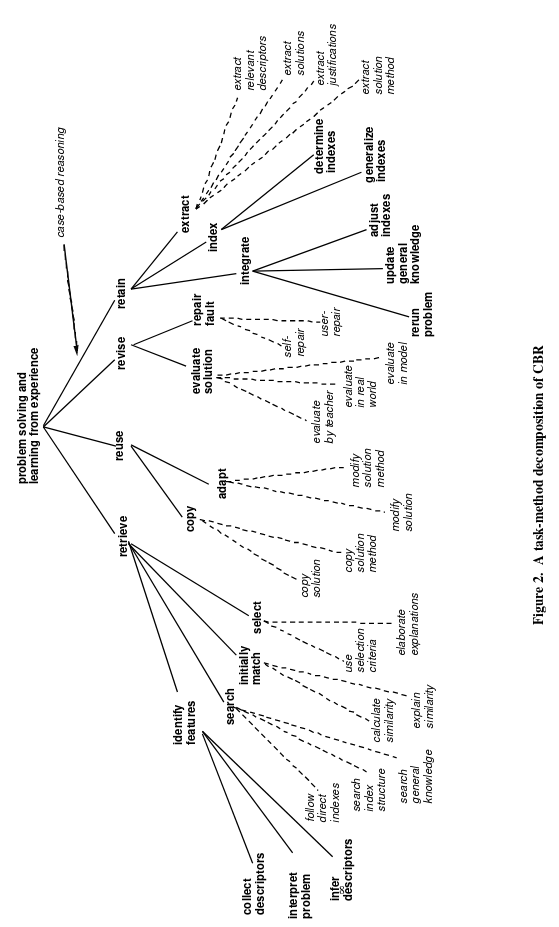
\includegraphics[scale=0.75, angle=270]{task_meth_decomp}
\end{figure}
\end{quote}

There are 5 problem areas that a CBR methods must have coherent solutions for to
be called a CBR:
\begin{itemize}
\item Knowledge representation
\item Retrieval method
\item Reuse method
\item Revise method
\item Retain method
\end{itemize}

\section{Representation of cases/Knowledge representation}
CBR uses past cases to solve new ones, so representing past cases(knowledge
base) in a way that makes searching it both effective and time efficient, is key.
It is also important to store new cases and solutions. From this the main
representation problem in CBR
becomes what to store in a case, how the cases content should be structured,
how all the cases should be organised/indexed for effective retrival and reuse,
and how general domain knowledge can be integrated into this structure. The
paper reviews two models; The dynamic memory model of Schank and Kolodner, and
the category-exemplar model of Porter and Bareiss.

\begin{quote}
\subsection{The Dynamic Memory Model} \label{subsec:dynamic_model}
The dynamic memory model is a hierarchical structure of episodic memory
organisation packets. It organises specific cases with simialar properties under
a general structure(a generalized episode - GE), this episode contains three
different types of objects: Norms, cases, and indices. The norms are the common
features of all the cases of a GE and the indices are the distinct features for
each case. And an index works like index do work, an index name and index value
and points to either a GE or a specific case. Searching in the tree is done by
``pushing down'' the case through the network structure. The model is
dynamic in the sense that when a new case is to be stored, it is again ``pushed
down'' through the network and if it ends up with the same index as another a
new GE is created. It is claimed that this model is suitable for learning both
generalized and case specific knowledge and that it is a model of human
reasoning and learning.

\begin{figure}
  \floatbox[{\capbeside\thisfloatsetup{capbesideposition={right,top},capbesidewidth=4cm}}]{figure}[\FBwidth]
  {\caption[Structure of the Dynamic Memory Model]{Structure of the dynamic
    model. It constructs a tree where each node is a GE with norms that are
    further seperated into indexes. Each index-value pair points from one GE to
    either a new GE or a case.}
  \label{fig:dynamicmodel}}
  {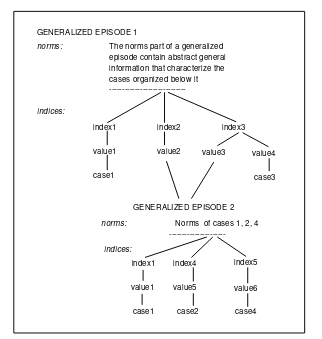
\includegraphics{dynamic_model}}

\end{figure}

\subsection{Category \& Exemplar Model} \label{subsec:cat_exem_model}
The idea behind this model is that real world/natural concepts should be defined
extensionally and that different features are assigned different importance' to
a case's membership to a category. The case memory is embedded in a network
structure of categories, semantic relations, cases and index pointers. Similar to
the dynamic model a index pointer may point to either a category or a case. The
indices are one of three types: feature links(pointing from features to
categories), case links(pointing from categories to cases/categories) and
difference links(pointing between similar cases). The cases of a category is
stored according to how ``typical'' of that category they are(their
prototypicality). Case matching(searching) is done by entering the new case's
features and returning the most prototypical cases of the matching category.
Similar to searching, a new case is stored by finding a matching case and creating
the appropriate feature indices. If the case is sufficiently similar to an
already existing case, it might not be retained at all, or merged with the
matching case.

\begin{figure}
  \floatbox[{\capbeside\thisfloatsetup{capbesideposition={right,top},capbesidewidth=4cm}}]{figure}[\FBwidth]
  {\caption[Structure of the Category \& Exemplar model]{Structure of the
      Category \& Exemplar model.}
  \label{fig:exemplarmodel}}
  {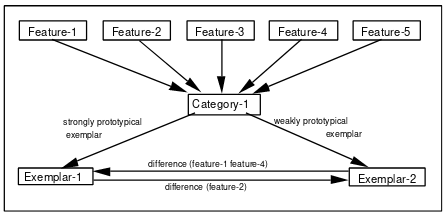
\includegraphics{cat_exemplar_model}}

\end{figure}

\end{quote}

\section{Case retrival}
The Retrive method takes a problem description and returns a best matching
previous case. It is split into 4 subtasks;
\begin{itemize}
\item Identify Features: Identify a new case's features/problem descriptors for
  use to match similar previous cases.
\item Initial Match: take the features found in the previous task and return a set of
  similar cases.
\item Search: A more elaborate search to reduces the number of cases found initially.
\item Select: Chooses the best solution based on the cases found in previous task.
\end{itemize}

\section{Case Reuse}
The reuse of the retrieved case solution in the context of the new case focuses
on two aspects: (a) the differences  among  the  past  and  the  current  case,
and (b) what part of retrieved case can be transferred to the new  case.  The
possible  subtasks  of  Reuse  are  Copy and Adapt;
\begin{enumerate}
\item Copy: Just reuse the solution of a previous case, not considering (a) and (b)
\item Adapt: There are two ways to reuse past cases with adaption
  \begin{itemize}
  \item Transformational reuse: Reuse and adapt the past case solution
  \item Derivational reuse: Reuse and adapt the past \emph{ method } that
    constructed the past solution
  \end{itemize}
\end{enumerate}

\section{Case Revision}
When a solution from the reuse phase is not correct, an opportunity to learn from
the failure arises. This is seperated into two tasks;
\begin{itemize}
\item Evaluate solution: See the results of applying the solution to the environment.
\item Repair fault: Detect the errors of the current solution and
  retrieve/generate explanations for the errors. Use these to modify(repair) the
  solution and retain usefull knowledge if possible. Then repeat the revision
  untill the solution is valid.
\end{itemize}

\section{Case Retainment - Learning}
This phase is triggered by the outcome of the case revision phase and involves
selecting which information to retain, in what form it is retained, how to index
the case, and how to intgrate the case into the memory structure.
\begin{itemize}
\item Extraction: Incorperate the new case into the memory or generalize the
  chosen previous case by retaining information from the current case. This
  information being gather from the Reuse or Revision phase, as the solution
  method, not just the concrete solution.
\item Index: The choice of indexing method influences how the cases are
  structured(its search space). This is a knowledge acquisition problem and
  should be handled in the modeling step\footnote{As in the system modelling
    step}. For examples see Sections \ref{subsec:dynamic_model} and \ref{subsec:cat_exem_model}
\end{itemize}

\setcounter{section}{0}
\chapter{Deep learning}
A deep learning system is a neural network. Neurons\footnote{A neuron is basicly a
  function(called the activation function) that takes inputs from the previous
  nodes in the network, toghether with weights and possible biases and the
  functions output(aka the neurons output) is sent to the next layer of
  neurons.} are set up in several layers, where a number of inputs are sent in
to the first layer, and the last layer gives an output.

Its the best, deep learning(DL) systems have beaten records in image
recognition, speech recognition, predicting the activity of potential drug
molecules, analysing particle accelerator data, reconstructing brain circuits,
and predicting the effects of mutations in non-coding DNA on gene expression and
disease, and more.

\section{Supervised learning}
Here the system is trained using a data set of inputs and a class. It takes each
input and sends it through the system, and uses an \emph{error function},
also called \emph{objective function} or \emph{loss function}, to
calculate the error(or distance) between the desired output and the actual
output. This error is then used to modify the weights of the network, this in
effect nudges the network to be more accurate when given a ``similar'' problem.
This weight adjustment is done by calculating each weights gradient, which is a number
representing that weights impact on the error/objective function. When
classifing, usually the weighted sum of the outputs are used to find which
category the input belongs to using thresholds.

From early on linear(also called shallow) classifieres(networks with few neurons and layer, i.e. the
perceptron) could only classify simple linearly seperable problem
spaces\footnote{A linearly seperable problem is a problem where, if the
  input(feature vector) and the target(correct classification of that input) is
  plotted on a graph(this plot is the search space/problem space) the different
  classes can be seperated by lines.}. By using deeper(several layer) networks
this problem can be solved.

\section{Backpropagation}
This is the process where the gradient(derivate) of the error function is
calculated with respect to each weight. Given an example from the training set
of inputs and target, backpropagation is done by first sending the inputs through the
network, this is the \emph{feed forward} step, this gives an output from the
network that is compared with the target of the example. Then, working backwards from
the output layer the gradient is calculated for each weight in the layer and the
weight is updated. More formally the steps are:
\begin{enumerate}
\item Take inputs(the feature vector) $\vec{x} = \langle x_1,x_2,..x_d \rangle$
  and the target $y^*$.
\item Feed the inputs through the network, using the weighted sum of the outputs
  of the previous layer as inputs to each activation function of the next layer
  untill the prediction(output of the network) is calculated, $y$.
\item Calculate the error $E = y-y^*$
\item backpropagate the error:
  \begin{enumerate}
  \item TODO: Add backprop algorithm
  \end{enumerate}
\end{enumerate}

A system using the algorithm presented above is called a feedforward neural
network and are used to map fixed-sized inputs, to fixed-sized outputs, like
categorizing an image. The nodes/neurons not in the input or output layers are
called hidden nodes/neurons and are responsible for distorting the input in a
way that makes the categories linearly seperable by the last layer.

\section{ Convolutional neural networks }
CNN are an extention to regular neural networks that work well with multi
dimentional inputs(images as 2d or 3d arrays) and can be constructed to be
multidimentional(input, hidden and output layers have both a height and a
width). In a convolutional layer the input of each node in the layer isn't
connected to all the nodes of the previous layer, instead it takes inputs from
a group of the nodes of the previous layer. There are also pooling layers, that
work the same way, but instead of using an activation fuction like ReLU, it uses
statistical functions, like output the max of the input values, or the average.

By using groups of inputs, the network can recognise shapes in the input,
independent of location. For example, if the CNN can recognise a dog, it can
recognise it anywhere in the picture, not just in the place where the dog was
placed in the training set. Because of this, and the efficient use of GPUs,
since 2012 CNN has taken over for older, classical computer-vision systems.

\section{Distributed representations and language processing}


\section{Recurrent neural networks}

\end{document}